\documentclass{acm_proc_article-sp}

\usepackage[utf8]{inputenc}
\usepackage[T1]{fontenc}

\usepackage[activate=compatibility]{microtype}

% autoref command
\usepackage[pdftex,urlcolor=black,colorlinks=true,linkcolor=black,citecolor=black]{hyperref}
\def\sectionautorefname{Section}
\def\subsectionautorefname{Subsection}
\def\subfloatautorefname{Subfigure}

\usepackage[lofdepth,lotdepth]{subfig}

\usepackage{enumitem}

\usepackage{mathtools}

% give emph a normal fontsize
\let\oldemph\emph
\renewcommand{\emph}[1]{\oldemph{\fontsize{9}{9}\selectfont #1}}

% more readable footnote layout
\renewcommand{\footnotesize}{\fontsize{8pt}{10pt}}
\setlength{\footnotesep}{.5cm}

% todo macro
\usepackage{color}
\newcommand{\todo}[1]{\noindent\textcolor{red}{{\bf \{TODO}: #1{\bf \}}}}

% listings and Verbatim environment
\usepackage{fancyvrb}
\usepackage{relsize}
\usepackage{listings}
\usepackage{verbatim}
\newcommand{\defaultlistingsize}{\fontsize{8pt}{9.5pt}}
\newcommand{\inlinelistingsize}{\fontsize{8pt}{11pt}}
\newcommand{\smalllistingsize}{\fontsize{7.5pt}{9.5pt}}
\newcommand{\listingsize}{\defaultlistingsize}
\RecustomVerbatimCommand{\Verb}{Verb}{fontsize=\inlinelistingsize}
\RecustomVerbatimEnvironment{Verbatim}{Verbatim}{fontsize=\defaultlistingsize}
\lstset{frame=lines,captionpos=b,numberbychapter=false,escapechar=§,
        aboveskip=0.5em,belowskip=0em,abovecaptionskip=0em,belowcaptionskip=0em,
framexbottommargin=-1em,
        basicstyle=\ttfamily\listingsize\selectfont}

% use Courier from this point onward
\let\oldttdefault\ttdefault
\renewcommand{\ttdefault}{pcr}
\let\oldurl\url
\renewcommand{\url}[1]{\inlinelistingsize\oldurl{#1}}

% superscript for 1st, 2nd, etc.
%\newcommand{\superscript}[1]{\ensuremath{^{\textrm{#1}}}}
%\newcommand{\subscript}[1]{\ensuremath{_{\textrm{#1}}}}
%\newcommand{\th}[0]{\superscript{th}}
%\newcommand{\st}[0]{\superscript{st}}
%\newcommand{\nd}[0]{\superscript{nd}}
%\newcommand{\rd}[0]{\superscript{rd}}

% linewrap symbol
\definecolor{grey}{RGB}{130,130,130}
\newcommand{\linewrap}{\raisebox{-.6ex}{\textcolor{grey}{$\hookleftarrow$}}}

% more pleasing quote environment
\usepackage{tikz}
\newcommand*{\openquote}{\tikz[remember picture,overlay,xshift=-7pt,yshift=1pt]
     \node (OQ) {\fontfamily{fxl}\fontsize{16}{16}\selectfont``};\kern0pt}
\newcommand*{\closequote}{\tikz[remember picture,overlay,xshift=2pt,yshift=-4.5pt]
     \node (CQ) {\fontfamily{fxl}\fontsize{16}{16}\selectfont''};}
\renewenvironment{quote}%
{\setlength{\parindent}{1cm}\par\openquote}
{\closequote\vspace{-4.5pt}
}

\makeatletter
\let\@copyrightspace\relax
\makeatother

\begin{document}

\title{Getting the Bigger Picture -- Extracting Media Items Covering Events from Multiple Social Networks}

\numberofauthors{3}
\author{
\alignauthor
\textbf{Thomas Steiner}\\
	\affaddr{Univ. Polit\`{e}cnica de Catalunya}\\
	\affaddr{Department LSI}\\
	\affaddr{08034 Barcelona, Spain,}\\
	\affaddr{tsteiner@lsi.upc.edu}
\alignauthor
\textbf{Raphaël Troncy}\\
	\affaddr{EURECOM}\\
	\affaddr{06560 Sophia Antipolis}\\
	\affaddr{France}\\
	\affaddr{rtroncy@eurecom.fr}
\and
\alignauthor
\textbf{Ruben Verborgh}\\ 	
	\affaddr{Ghent University -- IBBT, ELIS}\\
	\affaddr{Multimedia Lab}\\
	\affaddr{9050 Ghent, Belgium}\\
	\affaddr{ruben.verborgh@ughent.be}
\alignauthor
\textbf{Joaquim Gabarró Vallés}\\
	\affaddr{Univ. Polit\`{e}cnica de Catalunya}\\
	\affaddr{Department LSI}\\
	\affaddr{08034 Barcelona, Spain,}\\
	\affaddr{gabarro@lsi.upc.edu}	
}

\maketitle

\begin{abstract}
Core contributions:
Social network and media hosting platform agnostic media item search, and search results alignment.
Search results semantic enrichment by putting microposts and media items in relation.
Cross-channel popularity analysis.
Visual clustering, photos contained in videos.
\end{abstract}

\category{H.3.4}{Information Systems}{Information Storage and Retrieval}[World Wide Web]
\category{H.3.5}{Online Information Services}{Web-based services}

\keywords{\todo{Keywords}}

\section{Introduction} \label{sec:introduction}

\section{Social Networks and Media Items}

\subsection{Social Networks vs. Hosting Platforms}
The boundary between social networks and media hosting platforms is fluid.
There are media hosting platforms where people can upload their content with optionally content viewers -- in a relation to the original uploader or not -- having the possibility to react in form of comments, or in form of likes or dislikes.
An example is YouTube.
There are social networks where people can update their status, post links to stories, or upload their content with necessarily viewers -- standing in a relation or not -- having the option to react.
An example is Facebook.
Finally, there are hybrid forms, where social networks -- typically via third party applications -- integrate with media hosting platforms.
An example is the TweetDeck for Twitter application and their integration with TwitPic.

\subsection{Media Item Extraction}

\subsection{API Access vs. Web Scraping}
An \emph{Application Programming Interface (API)} in the sense of Web-based API is a programmatic specification intended to be used as an interface by software components on client and server to communicate with each other.

\emph{Web scraping} is the process of automatically extracting information from websites.
Web scraping involves practical solutions based on existing technologies that are often entirely ad hoc.
Examples of such technologies are regular expressions or DOM parsing of Web pages into a DOM tree.

The difference to the somewhat related concept of \emph{screen scraping} is that screen scraping relies on the visual layout of a website, whereas Web scraping relies on the textual and/or hierarchical structure of websites.

Social networks today are very much perceived as ``walled gardens'', excellently illustrated by a cartoon by David Simonds~(\autoref{fig:DavidSimonds}).
As with Orwell, where some animals are more equal than others, some social networks are more walled than others.
Some social networks have full read and write access via specified APIs.
An example is Twitter.
Other social networks have read access via APIs.
An example is Google+.
Interestingly, some media hosting platforms have just write API support, however, no read support, which requires us to fall back to Web scraping the website in order to retrieve data.
An example is Img.ly.

\begin{figure}
\centering
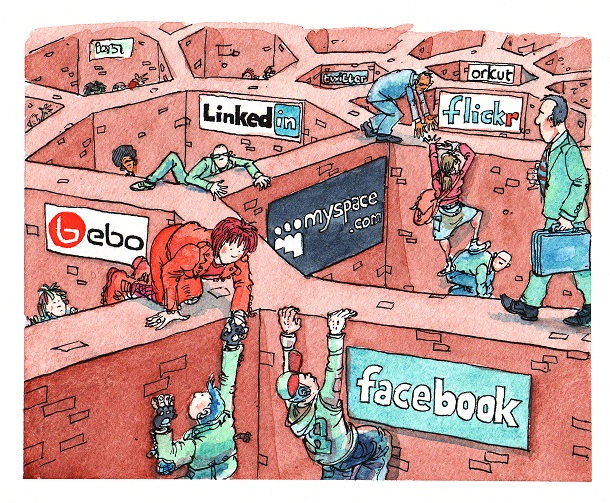
\includegraphics[width=1.0\linewidth,trim=16px 17px 12px 15px,clip]{./resources/davidsimonds.jpg}
\caption{David Simonds illustrates social networks as walled gardens due to their (by design) lock-in effects~\cite{DavidSimonds}.}
\label{fig:DavidSimonds}
\end{figure}

\section{Implementation Details}

\subsection{Data Structure}

\subsection{Media Item Collectors}

\subsection{Media Item Analysis}

\subsubsection{Machine Translation}

\subsubsection{Part of Speech Tagging}

\subsubsection{Named Entity Disambiguation}

\section{Experiments}

\subsection{Considered Events}

\subsubsection{Assad Speech}

\subsubsection{CES Las Vegas}

\subsubsection{Christian Wulff Case}

\subsubsection{Cut the Rope Launch}

\subsubsection{Dixville Notch}

\subsubsection{Free Mobile Launch}

\subsubsection{Ubuntu TV Launch}

\subsection{Discussion}

\section{Related Work} \label{sec:relatedwork}
\cite{Fabro2012}
Just Flickr and YouTube.
Use clustering algorithm for textual content.
Duplicate detection via Color and Edge Directivity Descriptor (CEDD).
Restrict selection to geolocated content and time period.

\cite{Liu2011}
Objective is to aggregate heterogeneous event information sources using Linked Data principles.
Just Flickr and YouTube.

\section{Future Work}

\section{Conclusion}

\section{Acknowledgments}
This work was partially supported by the European Commission under Grant No. 248296 FP7 \mbox{I-SEARCH} project.

% back to normal size Computer Modern for URLs in bibliography
\let\ttdefault\oldttdefault
\let\url\oldurl

\bibliographystyle{abbrv}
\bibliography{icmr2012}

\balancecolumns
\end{document}